\chapter{Конструкторский раздел}
\label{cha:design}

\section{Основные операции для работы с данными}

Разработанный метод распределенного хранения аудио-файлов в NoSQL-базе данных применяется на этапах добавления и извлечения аудио-файла из базы данных. 

\subsection{Добавление аудио-файла в MongoDB}

В процессе обработки операции записи данных в базу данных выполняется валидация глубины документа и проверка на наличие заданного клиентом идентификатора, а такаже присвоение идентификатора, в случае если его нет. Разработанный метод применяется на этом же уровне и состоит из следующих шагов.
\begin{enumerate}
\item Прверка на то, что данные являются MIDI-файлом (данные должны соответствовать определенной структуре, а также аудио-файл должен существовать и являться MIDI-файлом).
\item Извлечение пути к аудио-файлу и его имени для дальнейшего извлечения
\item Считывание содержимого аудио-файла.
\item Создание документа со специальной структурой (Parser).
\end{enumerate}

На рисунке 2.1 представлена функциональная декомпозиция этапов добавления аудио-файла в MongoDB.

\begin{center}
		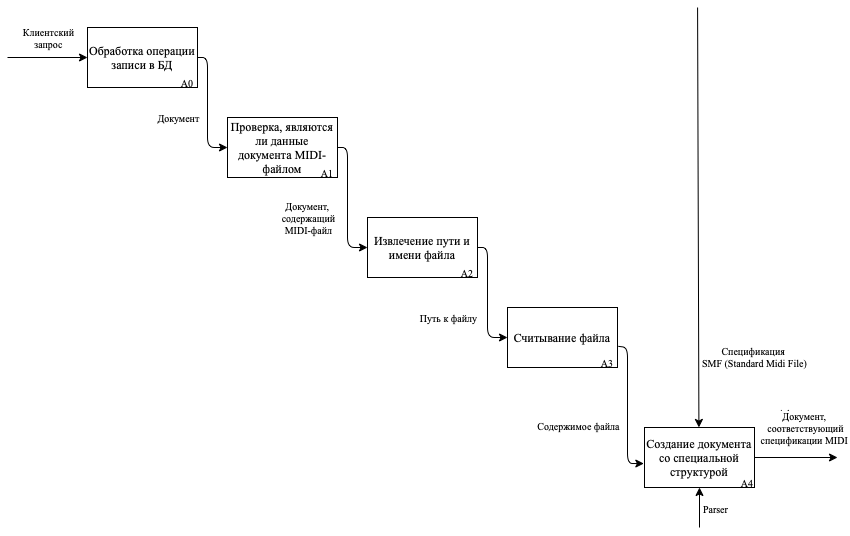
\includegraphics[scale=0.55]{tex/img/DecomposeInsert1.png}
		
			Рис 2.1 — Функциональная декомпозиция этапов добавления аудио-файла в MongoDB
\end{center} 

Формирование специальной структуры, соответствующей спецификации MIDI-файла, выполняется с помощью метода, представленного на листингах \ref{lst:parser_midi1} -- \ref{lst:parser_midi3}. Так как данные в MongoDB хранятся в виде объектов типа BsonDocument, весь MIDI-файл представлен в виде такого документа, где каждое поле является либо объектом типа BsonElement, либо, если имеет несколько полей, подобъектом типа BsonDocument, либо массивом подобъектов.

Тип BsonElement имеют следующие элементы MIDI-файла.

\begin{enumerate}
\item ID -- идентификатор заголовка MIDI (MThd) или музыкальной дорожки (MTrk). Тип данных: строка.
\item Length -- длина фрагмента заголовка или фрагмента музыкальной дорожки. Тип данных: бинарные данные.
\item Format -- формат MIDI-файла. Тип данных: бинарные данные.
\item NumTracks -- количество музыкальных дорожек. Тип данных: бинарные данные.
\item Devision -- разрешение MIDI-файла. Тип данных: бинарные данные.
\item Data -- данные музыкальной дорожки. Тип данных: бинарные данные.
\end{enumerate}
 
Также структура документа MongoDB, содержащего аудио-файл, была дополнена еще одним объектом типа BsonElement -- Name -- имя MIDI-файла, используемое при извлечении из базы данныхс опцией сохранения на диске. Тип данных: строка.

Тип BsonArray имеет поле <<MTrks>>, содержащее список объектов BsonDocument (каждый объект представляет одну музыкальную дорожку).

На рисунках 2.2 -- 2.5  представлена схема метода создания документа MongoDB по спецификации MIDI.

\begin{center}
		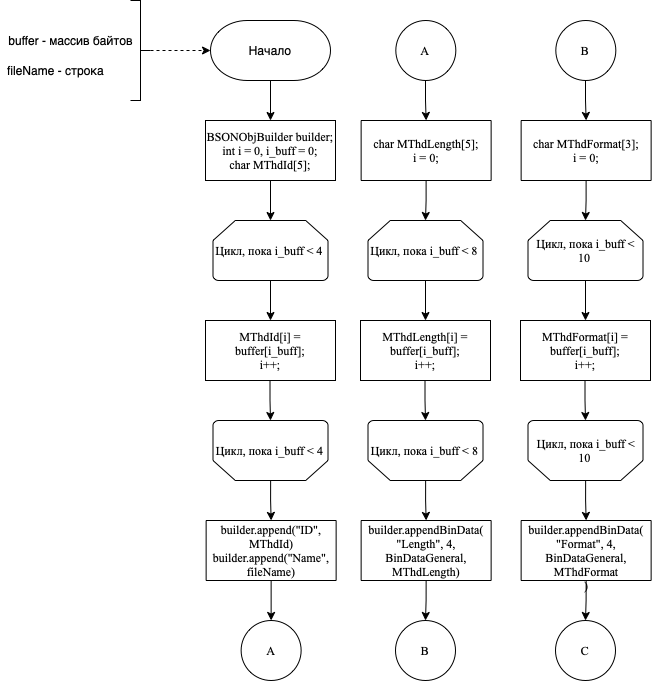
\includegraphics[scale=0.7]{tex/img/Parser1.png}
		
			Рис 2.2 — Схема метода создания документа MongoDB по спецификации MIDI (часть 1)
\end{center}

\begin{center}
		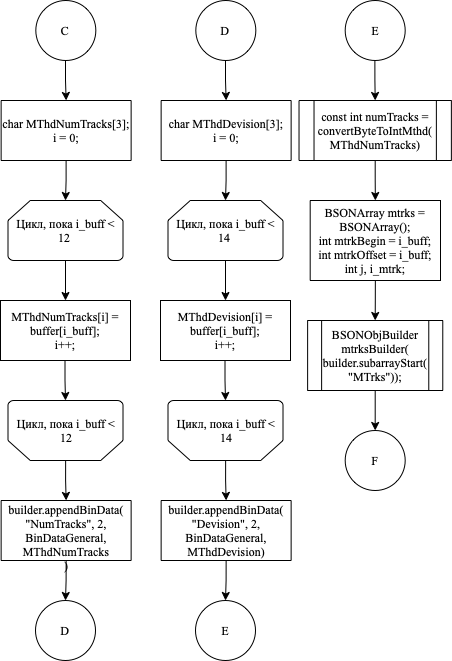
\includegraphics[scale=0.7]{tex/img/Parser2_1.png}
		
			Рис 2.3 — Схема метода создания документа MongoDB по спецификации MIDI (часть 2)
\end{center}

\begin{center}
		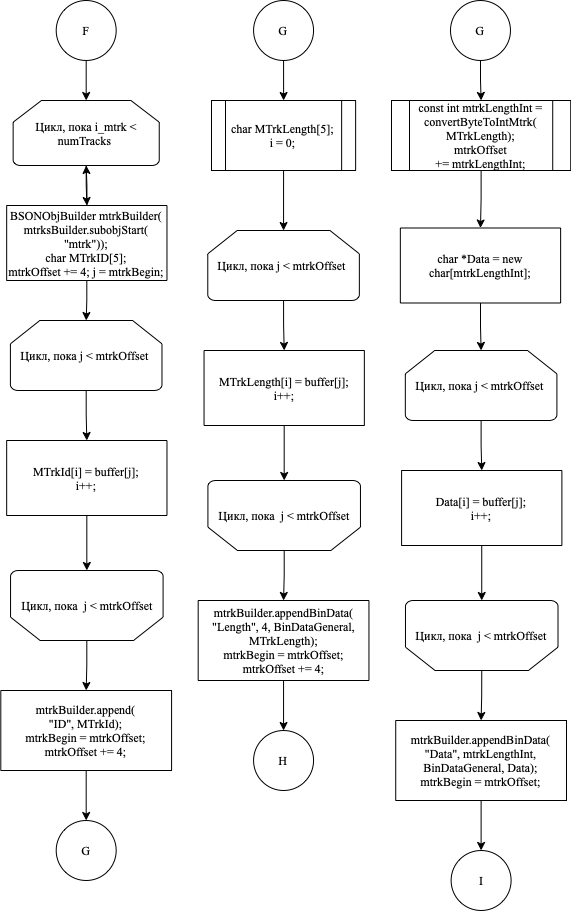
\includegraphics[scale=0.7]{tex/img/Parser3_1.png}
		
			Рис 2.4 — Схема метода создания документа MongoDB по спецификации MIDI (часть 3)
\end{center}

\begin{center}
		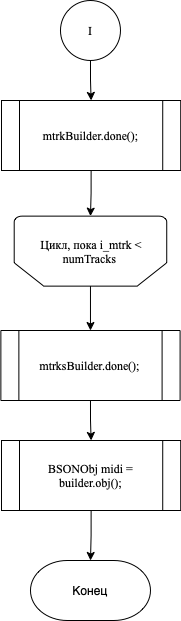
\includegraphics[scale=0.7]{tex/img/Parser4-2.png}
		
			Рис 2.5 — Схема метода создания документа MongoDB по спецификации MIDI (часть 4)
\end{center}

\subsection{Извлечение аудио-файла из MongoDB}

В ходе выполнения операции извлечения документа или набора документов из базы данных записи, содержащие MIDI-информацию, обрабатываются особым образом. Извлечение документа, имеющего структуру MIDI-файла, дополняется опцией сохранения данных локально в виде аудио-файла. После того как к запросу на извлечение данных применяется парсинг системы, извлекающий данные запроса, выполняется извлечение фильтра запроса и проверяется наличие в нем поля MidiSave, являющегося флагом, сигнализирующим о желании пользователя сохранить струкутуру MIDI-файла локально в формате аудио-файла с расширением <<.mid>>. Затем, когда запрос будет выполнен, в случае если в фильтре запроса есть поле MidiSave и оно имеет значение True, сохранение метода осуществится в три этапа.
\begin{enumerate}
\item Прверка на то, что данные являются MIDI-файлом (данные должны
соответствовать определенной структуре).
\item Формирование массива байтов из документа.
\item Запись массива байтов в файл.
\end{enumerate}

На рисунке 2.6 представлена функциональная декомпозиция этапов извлечения аудио-файла из MongoDB (если документ MongoDB необходимо сохранить в виде аудио-файла).

\begin{center}
		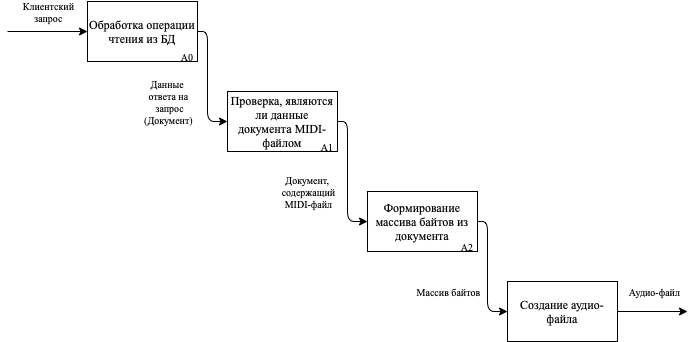
\includegraphics[scale=0.55]{tex/img/DecomposeFind.png}
		
			Рис 2.6 — Функциональная декомпозиция этапов извлечения аудио-файла из MongoDB (в случае записи документа MongoDB на диск в виде аудио-файла)
\end{center} 

Если в фильтре запроса нет поля MidiSave или оно имеет значение False, документ MongoDB не будет представлен в виде MIDI-файла и будет только возвращен клиенту в стандратном виде BsonDocument.

На рисунках 2.7 -- 2.9  представлена схема метода воссоздания MIDI-файла из документа MongoDB (листинги \ref{lst:file_builder1} -- \ref{lst:file_builder2}).

\begin{center}
		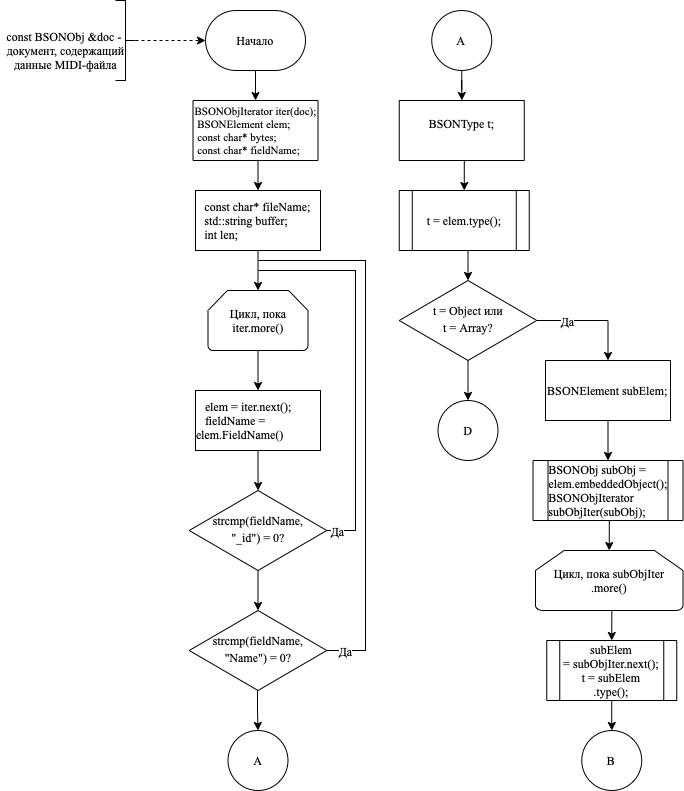
\includegraphics[scale=0.65]{tex/img/FileBuilder1.png}
		
			Рис 2.7 — Схема метода воссоздания MIDI-файла из документа MongoDB (часть 1)
\end{center}

\begin{center}
		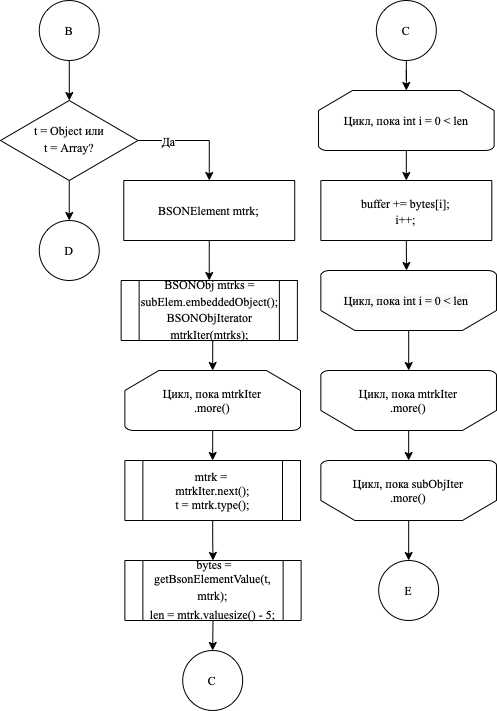
\includegraphics[scale=0.7]{tex/img/FileBuilder2.png}
		
			Рис 2.8 — Схема метода воссоздания MIDI-файла из документа MongoDB (часть 2)
\end{center}

\begin{center}
		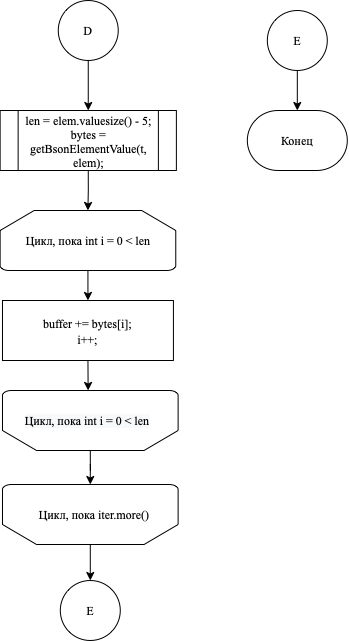
\includegraphics[scale=0.7]{tex/img/FileBuilder3.png}
		
			Рис 2.9 — Схема метода воссоздания MIDI-файла из документа MongoDB (часть 3)
\end{center}

\section{Ограничения предметной области}

Ограничения предметной области включают следующие пункты.

\begin{enumerate}
\item Добавление MIDI-файла в MongoDB и извлечение документа с его последующей записью на диск в формате MIDI-файла имеют жестко заданные API.
\begin{enumerate}
\item API записи аудио-файла в базу данных включает в себя все команды вставки, но имеет строгую структуру, представленную на листинге \ref{lst:insert_structure}, где path -- это путь к аудио-файлу, а name (может быть опущено) -- имя файла, используемое при сохранении документа в формате MIDI файла. Если эта структура не будет соблюдена, вставки аудио-файла в базу в предусмотренном в разработанном методе формате не произойдет.
\item API чтения аудио-файла из базы данных включает в себя все команды чтения, но для сохранения документа в виде аудио-файла необходимо задать поле MidiSave фильтра запроса, установив ему значение True.
\end{enumerate}
\item Пользователь не имеет возможности задавать тип данных, в котором будут храниться поля аудио-файла в базе данных.
\item Данные, представляющие музыкальную дорожку, не разбиваются на логические подструктуры.
\end{enumerate}

\begin{lstlisting}[language=C, label=some-code, caption=Структура запроса на добавление аудио-файла в MongoDB, label=lst:insert_structure]
{ 
    path: string("some data"),
    name: string("some data")
}
\end{lstlisting}

\section{Выводы из конструкторского раздела}

В данном разделе были описаны основные операции для работы с данными при использовании разработанного метода распределенного хранения аудио-файлов в NoSQL-базе данных, была проведена функциональная декомпозиция этих операций, были представлены схемы работы метода, реализующего создание документа MongoDB, соответствующего спецификации MIDI, из сырого содержимого аудио-файла. Также были определены ограничения предметной облвсти.
%%% Local Variables:

%%% mode: latex
%%% TeX-master: "rpz"
%%% End:
%--количество цветов
%||количество пикселей